\chapter{Related Work} \label{cha:related_work}

\section{Context}

The following chapter provides context about to the challenge we attempt to solve and presents the identified sub-challenges towards performing management of microservices in the edge of the network. 

First, \textbf{microservice networking}: microservices need to cooperate towards solving applicational tasks, as such, peers in the system need to be integrated in an efficient abstraction layer that allows them to find each other and communicate. This raises an old challenge in P2P computing: how can peers organize themselves in the network such that they can find resources (e.g. other peers, services or even computing power) in an efficient way? It is important to notice that the edge environment is composed by lots of sub-networks composed of heterogenous devices concurrently entering and leaving the network, which presents a hard scenario in \textbf{resource location systems}, particularly in performing \textbf{topology management}, because the overlay needs to federate large numbers of devices and adapt to the underlying network in order to remain efficient. 

Addressing this, section \ref{sec:topology_management} of this chapter provides context about \textbf{topology management}, particularly the main categories of topologies and discuss their applicability in edge environments. Second section, \ref{sec:res_location} covers \textbf{resource location architectures}, which leverage on one (or a combination of) topologies to index resources in the system. For each type of architecture we discuss their differences and present popular implementations in the state of the art. 

Provided that we have an efficient overlay that we can employ towards deploying microservices, the next step is \textbf{ensuring and maintaining quality of service}. For this, we need to perform \textbf{monitoring} of device and service status, with a special emphasis on devices in the edge environment. Section \ref{sec:res_monitoring} covers popular techniques used towards tracking device and service status, we particularly study which metrics to collect that assist in pinpointing causes of QoS degradation. Furthermore, section \ref{sec:res_monitoring} also covers related work about monitoring edge devices and some examples of popular monitoring systems.

However, if we wish to gather metrics on device and service status, devices will produce a continuous stream of monitoring data, transmitting and storing that data becomes a limitation to the scalability of the system. To circumvent this, that data needs to somehow be combined, this is called \textbf{aggregation}. Section \ref{sec:aggregation} studies aggregation, which consists in the process of combining several numeric values into one single representative \cite{grabisch2009aggregation}. Next, we discuss the different types of aggregation, and how they can be applied towards maintaining the aforementioned quality of service.

Lastly, section \ref{sec:offloading_computation} studies how the aggregated results can be used to perform microservice management and deployment. Namely, how to orchestrate microservices such that the computation is offloaded to the Edge. We discuss paradigms such as Fog Computing and Osmotic Computing and how they compare to Edge Computing. Lastly, we discuss approaches towards implementing elastic computing in Edge environments.

\section{Topology Management} \label{sec:topology_management} 
% -------------------
% Topology Management
% -------------------



Provided with an overview of the taxonomy of the devices materializing edge environments, we now study the related work towards federating all these devices (that we also refer to as peers following the peer-to-peer (P2P) literature nomenclature) in an abstraction layer (an overlay network) that allows intercommunication, cooperation, and efficient resource discovery \cite{leitaoPHDthesis}. This Section provides context regarding the taxonomy of overlay networks, followed by a discussion of popular overlay network protocols and what we believe to be their strengths and limitations.

In a P2P system, peers contribute to the system with a portion of their resources to accomplish tasks otherwise unfeasible by an individual peer. Typically, this is achieved in a decentralized way, which means peers must establish neighbouring connections among themselves to enable information exchange which, in turn, enables progress towards the system goals. 

Participants in a P2P system may know all other peers in the system, which is typically referred to as \textbf{full membership} knowledge, which is a popular approach in Cloud systems. However, as the system scales to larger numbers of peers, concurrently entering and leaving the system (a phenomenon called churn \cite{stutzbach2006understanding}), this information becomes costly to maintain up-to-date. 

In order to circumvent the aforementioned challenges, a common alternative is to have peers only maintain a view of a subset of all peers in the system, which is called \textbf{partial membership}. This information is maintained by some membership algorithm that restricts neighbouring relations among peers. Partial membership solutions are attractive because they offer similar functionality to full membership systems while achieving more scalability and resiliency to churn. The closure of these neighbouring relations is what materializes an \textbf{overlay network}, a logical (i.e. at the applicational level) network that is defined above another network (e.g. the IP network).

\subsection{Taxonomy of Overlay Networks}

Overlay networks are logical networks that operate at the applicational level. These rely on an existing network (commonly referred to as the \textit{underlay}) to establish neighbouring relations, where each participant typically only communicates directly with its overlay neighbours \cite{leitaoPHDthesis}. Overlays are commonly designed towards specific applicational needs. As such, their neighbouring relations may or may not follow some established logic. As illustrated in Figure \ref{fig:overlay_networks}, there are two main categories of overlays: \textbf{structured} and \textbf{unstructured}:

\subsubsection*{Unstructured Overlays}

\begin{figure}
    \centering
    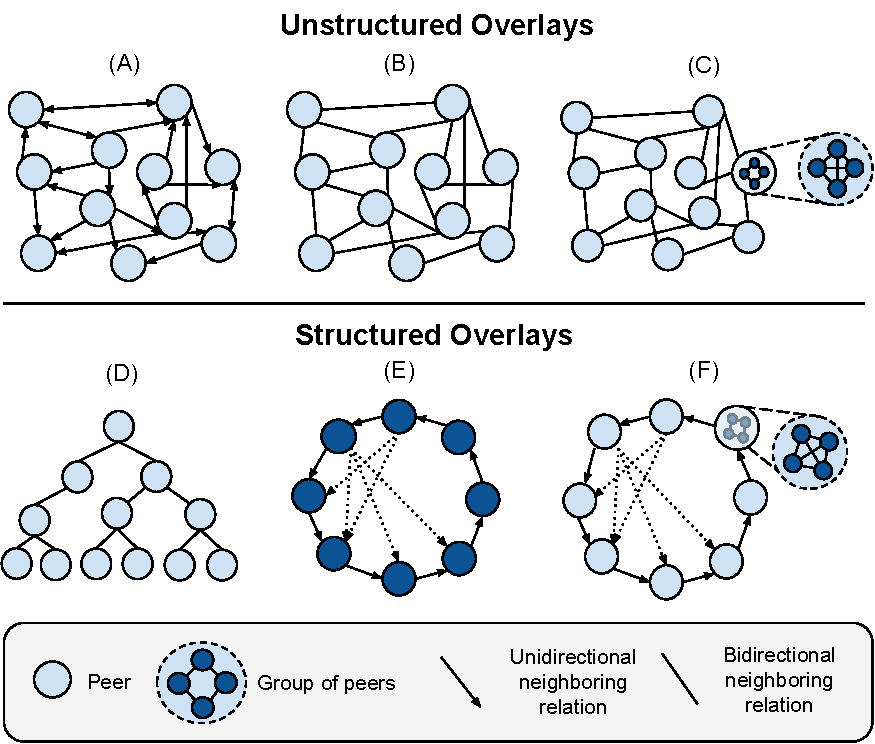
\includegraphics[width=0.60\linewidth]{Chapters/Figures/overlay_networks.pdf}
    \caption{Examples Overlay Networks}
    \label{fig:overlay_networks}
\end{figure}

Unstructured overlays usually impose little to no rules in neighbouring relations. Nodes may pick random peers to be their neighbours or employ strategies to rank neighbours and selectively pick the best given particular criteria typically entwined with the needs of applications. A key factor of unstructured overlays is their low maintenance cost, given that nodes can easily create neighbouring relations, which eases the process of replacing failed ones. Consequently, this is the type of overlay which offers better resilience to churn.

In Figure \ref{fig:overlay_networks}, we illustrate three examples of unstructured overlay networks: (A) is a representation of an overlay network where the connections are unidirectional (e.g. Cyclon \cite{jelasity2007gossip}), in this type of overlay, peers have no control over the status of incoming connections. Consequently, a peer may become isolated from the network without realizing it, which is undesirable. 

Overlay (B) is similar to (A), however, its neighbouring connections are bidirectional. This means that a peer with a given number of outgoing connections must also have the correspondent number of incoming connections, diminishing the risk of the peer becoming disconnected from the overlay (this is the approach taken by HyParView \cite{Hyparview} to achieve high reliability and fault-tolerance).

Lastly, (C) is a representation of an unstructured overlay where peers establish groups among themselves (such as Overnesia \cite{leitao2014overnesia}). Grouping multiple devices into a group can provide benefits such as (1) failures can be quickly identified and resolved by other members of the group; (2) nodes can replicate data within the group, leading to increased availability of that data; (3) groups can abstract groups of resources and internally manage their usage by, for example, offloading computational tasks within the group in a localized way. 

\subsubsection*{Structured Overlays}

Structured overlays enforce stronger rules towards neighbour selection (generally based on the identifiers of peers). As a result, the overlay generally converges to a certain topology known a \textit{priori} (e.g., a ring, tree, hypercube, among others). 

Figure \ref{fig:overlay_networks} also illustrates three kinds of structured overlay networks: (D) corresponds to a tree, which are widely used to perform broadcasts (e.g., PlumTree \cite{plumTree}) because of the smaller message complexity required to deliver a message to all nodes, or to monitor the system state (if nodes in lower levels of the tree periodically send monitoring information \cite{leitao2008large} to upper levels in the tree, in turn, the root of the node has a global view of the collected monitoring information (e.g., Astrolabe \cite{Renesse2003})). However, trees are very fragile in the presence of faults \cite{plumTree}.

Overlay (E) corresponds to an overlay typically expected to define Distributed Hash Tables (DHTs). These are extremely popular due to their effective applicational-level routing capabilities. In a DHT, peers employ a global coordination mechanism that restricts their neighbouring relations such that they can find any peer \textit{responsible} for any given key in a  limited number of steps (typically the logarithm of the system size). In this example (figure E), the topology consists of a ring (which is the strategy employed by Chord \cite{stoica2003chord}). It is important to mention that not all distributed hash tables rely on rings to perform effective routing. For example, in Kademlia \cite{maymounkov2002kademlia}, nodes organize as leaves across a binary tree.

Finally, the overlay denoted in (C) is similar to overlay (E), however each position of the DHT is made up of a virtual node composed of multiple physical nodes (which is the strategy employed by Rollerchain \cite{rollerchain}). Because of this, routing procedures are still limited acording to the logarithm of system size, and also have the potential to be load-balanced. Furthermore, as the failure of a physical node does necessarily mean the failure of a virtual node, churn effects are mitigated. 
 
\subsection{Overlay Network Quality Metrics}

If we look at an overlay network where connections between nodes represent edges and nodes represent vertices in a graph, we obtain a graph from which we may extract direct metrics to estimate overlay performance \cite{leitaoPHDthesis}, we now enumerate some which we believe to be the most relevant to our goal:

\begin{enumerate}
    
    \item \textbf{Connectivity}. This property is usually measured as a percentage, corresponding to the largest portion of the system that is connected, intuitively, a connected graph is one where there is at least one path from each node to all other nodes in the system.
    
    \item \textbf{Degree Distribution}. The degree of a node consists in the number of arcs that are connected to it. In a directed graph, there is a distinction between \textbf{in-degree} and \textbf{out-degree} of a node, nodes with a high in-degree value have higher reachability, while nodes with 0 in-degree cannot be reached. The out-degree of a node represents a measure of the contribution of that node towards the maintenance of the overlay topology.
    
    \item \textbf{Average Shortest Path}. A path is composed by the edges of the graph that a message would have to cross to get from one node to other. The average shortest path consists in the average of all shorter paths between every pair of peers, to promote efficient communication patterns, is desirable that this value is as low as possible.
    
    \item \textbf{Clustering Coefficient}. The clustering coefficient provides a measure of the density of neighbouring relations across the neighbours of links between a given node. It consists in the number of a node's neighbours divided by the maximum number of links that could exist between those neighbours. A high value of clustering coefficient means that there is a higher amount of redundant communication among nodes.
    
    \item \textbf{Overlay Cost}. If we assume that a link in the overlay has a \textit{cost}, (e.g. derived from latency), then the overlay cost is the sum of all the costs of the links that form the overlay. 
    
\end{enumerate}

\subsection{Relevant examples of Overlay Networks}

\textbf{T-MAN} \cite{t-man} is a protocol to manage the topology of overlay networks, it is based on a gossiping scheme, and proposes to build a wide range of structured overlay networks (e.g., ring, mesh, tree, among others). To achieve this, T-MAN expects a cost function as an input to the protocol, then employed as a ranking method, applied iteratively by every node to compare the preference among possible neighbours. 

Nodes periodically exchange their neighbouring sets with peers in the system and keep the nodes which rank higher according to the ranking method. A limitation of T-Man is that it does not ensure the stability of the in-degree of nodes during the optimization of the overlay, and consequently, the overlay may not remain connected. 

\textbf{Management Overlay Network} \cite{liang2005mon} (MON) is an overlay network system aimed at facilitating the management of large distributed applications. This protocol builds on-demand overlay structures that allow users to execute instant management commands, such as query the current status of the application or push software updates to all the nodes. MON performs these procedures in an on-demand fashion such that it achieves a low maintenance cost when no commands are running.

This solution allows the on-demand construction of two types of Overlay Networks: trees and direct acyclic graphs. These overlays, in turn, can be employed towards aggregating monitoring data related to the status of the devices. Limitations from using MON are that the resulting overlays are susceptible to topology mismatch, and do not ensure connectivity. Furthermore, since the topologies are supposed to be short-lived, MON does not provide mechanisms for dealing with faults.

\textbf{Hyparview} \cite{Hyparview} (Hybrid Partial View) gets its name from maintaining two exclusive views: the \textit{active} and \textit{passive} view, which are distinguished by their size and maintenance strategy. 

The \textit{passive view} is a larger view which consists of a random set of peers in the system,  maintained by a periodic gossip protocol, where each peer sends a message to another random peer in their active view. This message contains a subset of the neighbours of the sending node and a time-to-live (TTL). The message is then forwarded randomly throughout the system until the TTL expires, updating the views of nodes it passes. In contrast, the \textit{active view} consists of a smaller view (around log(n) in size), created during the bootstrap of the protocol. Each peer in the view has an associated TCP connection, which is then used as a bidirectional connection medium and failure detector. Whenever a node from the active view is detected as failed, it is replaced with one in the passive view.

Hyparview is often used as a \textit{peer sampling service} for other protocols which rely on the connections from the active view to collaborate (e.g. PlumTree \cite{plumTree}). It achieves high reliability even in the face of a high percentage of node failures. However, its resulting topology is flat, which we believe to not be ideal for the taxonomy of edge environments we are considering. Furthermore, it may suffer from topology mismatch: given the random nature of neighbouring connections, the resulting neighbouring connections may be very distant in the underlying network.

\textbf{X-BOT} \cite{x-bot} is a protocol that constructs an unstructured overlay network where neighbouring relations are biased considering one metric. This metric is provided by an \textit{oracle}, which is a component that exports a function, which accepts a pair of peers and attributes a cost to that neighbouring connection. This cost may take into consideration factors such as latency, ISP distribution, network stretch, among others. 

The rationale X-BOT is as follows: nodes maintain active and passive views similar to Hyparview \cite{Hyparview}. Then, nodes periodically trigger optimization rounds where they attempt to bias a portion of their connections according to the functions provided by the oracle. Although this protocol potentially addresses the previous concerns about the overlay topology mismatching the underlying network, it still proposes a flat topology, which, as previously mentioned, we believe is not adequate for the edge environment taxonomy. 

\textbf{Overnesia} \cite{leitao2014overnesia} is a protocol that establishes an overlay composed of fully connected groups of nodes, where all nodes within a group share the same identifier. Nodes join the system by sending a request to a bootstrap node, triggering a random walk. The requesting node joins the group where its random walk terminates (either because it finds an underpopulated group or because the TTL expires). 

Nodes enforce intra-group membership consistency through an anti-entropy mechanism where nodes within a group periodically exchange messages containing their view of the group. When a group detects that its size has become too large, it triggers a dividing procedure that splits the group in two halves. Conversely, when the group size has fallen below a certain threshold, nodes trigger a collapsing procedure. During it, each node takes the initiative to relocate itself to another group, resulting in the graceful collapse of the group. Finally, inter-group links are acquired by propagating random walks throughout the overlay.

As previously mentioned, establishing groups of nodes enable load-balancing, efficient dissemination of queries, and fault tolerance. Furthermore, it allows the abstraction of a set of physical resources into a single, unified, logical resource. 

However, in systems with heterogeneous composition, system scalability limitations may arise as devices may have trouble maintaining the group view up-to-date and the active connections to all group members. Finally, the overlay may suffer from topology mismatch, as two nodes within the same group may be distant within the underlay.

\textbf{Chord} \cite{stoica2003chord} is a well known structured overlay network where the protocol builds and manages a ring topology, similar to overlay (E) in Figure \ref{fig:overlay_networks}. Each node is assigned an m-bit identifier, uniformly distributed across the id space, and takes steps to fill its \textit{finger table}. The finger table contains at most \(m\) entries, each $ith$ entry of this table corresponds to the first peer that succeeds a certain peer \(n\) by \(2^{ith}\) in the ring. This means that whenever the finger table is up-to-date, and the system is stable, lookups for any data piece only take logarithmic time to finish. 

Although Chord provides a good trade-off between bandwidth and lookup latency, it has its limitations: peers do not learn routing information from incoming requests, links have no correlation to latency or traffic locality, and the overlay is highly susceptible to churn \cite{dht_performance_churn}. Finally, the ring topology is flat, which means that lower capacity nodes in the ring may become a limitation instead of an asset in the context of routing procedures.

%Chord is the building block for many other solutions: Cyclone \cite{Artigas2005} is a hierarchical DHT inspired on Chord which constructs clusters by splitting the ID space into a PREFIX and SUFIX. The PREFIX provides intra-cluster identity, whereas the SUFIX lets nodes know their residence cluster.

%Hieras \cite{1240580} uses a binning scheme according the underlay topology to group peers into smaller rings. The lower the ring, the smaller the average link latency. Routing is done in lower rings to make use of the reduced latency and if the resource is not present in those rings, then the query is forwarded to higher rings.

%Crescendo \cite{Ganesan2004} splits the ID range into domains (similar to DNS), where nodes in leaf-domains form Chord rings, then nodes merge rings by applying rules such that rings in different domains can communicate. The resulting routing table and the routing procedures in Crescendo are similar to Chord.

\textbf{Pastry} \cite{rowstron2001pastry} is another well known DHT which assigns a 128-bit node identifier (nodeId) to each peer in the system. The nodeIds are randomly generated, and consequently, are uniformly distributed in the 128-bit nodeId space. Routing procedures are forwarded to nodes whose nodeId shares a prefix that is at least one bit closer to the key, if there are no nodes available, nodes route messages towards the numerically closest nodeId. This routing procedure takes O(log N) routing steps, where N is the number of Pastry nodes in the system. 

This protocol has been widely used as a building block for Pub-Sub applications such as Scribe \cite{10.1007/3-540-45546-9_3} and file storage systems like PAST \cite{990064}. However, limitations from using Pastry arise from the use of a numeric distance function towards the end of routing procedures, which creates discontinuities at some nodeId values and complicates attempts at formal analysis of worst-case behaviour, in addition to establishing a flat topology that mismatches the edge device taxonomy.

\textbf{Tapestry} \cite{tapestry} Is a DHT with similar behaviour to Pastry~\cite{rowstron2001pastry}. In this system, however, nodeIDs are represented using base b, where b is a parameter specified during configuration. In routing procedures, messages are incrementally forwarded to the destination digit by digit (e.g. ***8 -> **98 -> *598 -> 4598). Consequently, in stable conditions, routing procedures theoretically take $\log{b}{n}$ hops to reach their destination, where b is the base of the ID space. Because nodes assume that the preceding digits all match the current node's suffix, nodes in Tapestry only need to keep a constant size of $\log{N}$ entries at each route level, consequently, nodes contain entries for a fixed-sized neighbour map of size b.  

\textbf{Kademlia} \cite{maymounkov2002kademlia} is a DHT where nodes are considered leaves distributed across a binary tree. Peers route queries and locate data pieces by employing an XOR-based distance function which is symmetric and unidirectional. Each node in Kademlia is a router where its routing tables consist of shortcuts to peers whose XOR distance is between \(2^{i}\) by \(2^{i + 1}\) in the ID space, given the use of the XOR metric, "closer"\ nodes are those that share a longer common prefix.

The main benefits that Kademlia draws from this approach are: nodes learn routing information from receiving messages, there is a single routing algorithm for the whole routing process (unlike Pastry \cite{rowstron2001pastry}) which eases formal analysis of worst-case behavior. Finally, Kademlia exploits the fact that node failures are inversely related to uptime by prioritizing nodes that are already present in the routing table.

\textbf{Kelips} \cite{gupta2003kelips} is a group-based DHT which exploits increased memory usage and constant background communication to achieve reduced lookup time and message complexity. Kelips nodes are split in $k$ affinity groups split in the intervals [0,$k-1$] of the identifier space, thus, with $n$ nodes in the system, each affinity group contains $\frac{n}{k}$ peers. Within a group, nodes store a partial set of nodes contained in the same affinity group and a small set of nodes lying in foreign affinity groups. With this architecture, Kelips achieves O(1) time and message complexity in lookups, however, it has limited scalability when compared to previous DHTs, given the increased memory consumption (O($\sqrt{n}$).

\textbf{Rollerchain} \cite{rollerchain} is a protocol which establishes a group-based DHT by leveraging on techniques from both structured and unstructured  overlays (Chord and Overnesia). In short, the Overnesia protocol materializes an unstructured overlay composed by logical groups of physical peers who share the same identifier. Then, the peer with the lowest identifier within each logical group joins a Chord overlay, obtains the adresses of other virtual peers, and distributes them among group members.

Rollerchain has the potential to enable a type of replication which has higher robustness to churn events when compared to other other replication strategies, however, there are limitations to this approach: (1) the load is unbalanced within members of each group, as only one node is in charge of populating and balancing the inter-group links; (2) similar to Chord, nodes do not learn from incoming queries, which contrasts with other DHTs such as Pastry; (3) the protocol has a higher implementation complexity and maintenance cost when compared to a regular DHT.

\subsection{Discussion}

Unstructured overlays are an attractive option for federating large amounts of devices in heavily dynamic environments. They provide a low clustering coefficient, are flexible, and maintain good connectivity even in the face of churn. However, given their unstructured nature, they are limited in certain scenarios, for example, when trying to find a specific peer or resource in the system.

Conversely, distributed hash tables enable efficient routing procedures with very low message overhead, which makes them suitable for application-level routing. However, given their strict neighbouring rules, participating nodes cannot replace neighbours easily, which hinders the fault-tolerance of these types of topologies, in addition, given the fact that devices in edge environments have varied computational power and connectivity, they may become a limitation instead of an asset in the context of routing procedures. 

%Hierarchical DHTS consisting of DHTS contained within other DHTS (e.g. a ring within a ring) offer several advantages over a flat DHT: first, lookups take less hops and messages to reach the target, second, organizing nodes in disjoint groups allows traffic locality if groups of nodes are close within the underlay, and churn events within a group stay contained within that group. 

%However, many of these systems either employ more memory to accommodate the many levels of the hierarchy, or tradeoff reliability (by shortening the number of connections) for memory and communication efficiency. 

\section{Resource Location and Discovery} \label{sec:res_location} 
% resource management in the DC
% -------------------
% Resource Management
% -------------------

Resource location systems are one of the most common applications of the P2P paradigm \cite{leitaoPHDthesis}, in a resource location system, a participant provided with a resource descriptor is able to query other peers and obtain an answer to the location (or absence) of that resource in the system within a reasonable amount of time. To do so, resource location systems employ search strategies, which depend on : (1) the structure the an overlay network (structured or unstructured). (2) on the characteristics of the resources to search (e.g. if there are many copies of it or not), and (3) on the desired results (e.g. if a single copy of a resource satisfies the query, or multiple are required). 

In the context of resource management, if a peer wishes to offload computations to other peers, it must employ an efficient search strategy to find nearby available resources (e.g., storage capacity, computing power, among others) in order to offload computations. In this section, we cover resource location and discovery, starting with the taxonomy of querying techniques for P2P systems, followed by the study of how resources can be stored or indexed and looked up throughout the topologies studied in the previous section.

\subsection{Querying techniques}

Querying techniques consist of how peers describe the resources they need, these, according \cite{leitaoPHDthesis}, may be classified as: \textbf{(1)~Exact Match queries}, these specify the resource to search by the value of a unique attribute (i.e., an identifier, commonly the hash of the value of the resource); the second querying methodology type is \textbf{(2)~keyword queries}, that employ one or more keywords (or tags) combined with logical operators to describe resources (e.g. "pop", "rock", "pop and rock" ...); next, \textbf{(3)~range queries} retrieve all resources whose value is contained within a given interval (e.g. "movies with 100 to 300 minutes of duration"); finally, \textbf{(4)~arbitrary queries} aim to find a set of nodes or resources that satisfy one or more arbitrary conditions (e.g. looking for a set of resources encoded in a certain format).

Provided with a way of describing their resource needs, peers need strategies to index and retrieve the resources in the system, there are three popular techniques: \textbf{centralized}, \textbf{distributed over an unstructured overlay}, or \textbf{distributed over a structured overlay}.

\subsection{Centralized Resource Location}

\textbf{Centralized resource location} relies on one (or a group of) centralized peers that index all existing resources. This type of architecture greatly reduces the complexity of systems, as peers only need to contact a subset of nodes to locate resources. 

It is important to notice that in a centralized architecture, while the indexation of resources is centralized, the resource access may still be distributed (e.g. a centralized server provides the addresses of peers who have the files, and files are obtained in a pure P2P fashion), a system which employs this architecture with success is BitTorrent \cite{cohen2003incentives}.

Although centralized architectures are widely used nowadays, they lack the necessary scalability to index the large number of dynamic resources we intend to manage, and have limited fault tolerance to failures, making them unsuited for edge environments. 

%However, there are many ways that a hybrid architecture can be applied to Edge computing: since the failure rate of a single data center (DC) is low, if we assume a system composed by multiple DCs, they may act as a reliable failover for whenever edge devices are partitioned of fail. 

\subsection{Resource Location on Unstructured Overlays}

When employing an unstructured overlay for resource location, the resources are scattered throughout all peers in the system, consequently, peers need to employ distributed search strategies to find the intended resources. This is accomplished through disseminating messages containing these queries throughout the overlay. The dissemination of these messages can follow multiple strategies, we now cover there two popular approaches: \textbf{flooding} and \textbf{random walks} \cite{leitaoPHDthesis}. 

\textbf{Flooding} consists of peers eagerly forwarding queries to others in the system as soon as they receive them for the first time, the objective of flooding is to contact multiple distinct peers that may have the queried resource. One approach is \textbf{complete flooding}, which consists in contacting every node in the system, this guarantees that if the resource exists, it will be found. However, complete flooding is not scalable and incurs significant message redundancy. \textbf{Flooding with limited horizon} minimizes the message overhead by attaching a TTL to messages that limits the number of times a message can be retransmitted. However, there is a trade-off for efficiency: flooding with limited horizon does not guarantee that all resources will be found. 

\textbf{Random Walks} are a dissemination strategy that attempts to minimize the communication overhead that is associated with flooding. A random walk consists of a message with a TTL that is randomly forwarded one peer at a time throughout the network. Random walks may also attempt to bias their path towards peers that are more likely to have answers to the query \cite{1022239}, this technique is commonly reffered to in the literature as a \textbf{random guided walk}. A common approach to bias random walks is to use bloom filters \cite{5751342}, which are space-efficient probabilistic data structures that allow the creation of imprecise distributed indexes for resources.

First generation of decentralized resource location systems relied on unstructured overlays (such as Gnutella \cite{gnutella_gtk}) and employed simple broadcasts with limited horizon to query other peers in the system. However, as the size of the system grew, simple flooding techniques lacked the required scalability for satisfying the rising number of queries, which triggered the emergence of new techniques to reduce the number of messages per query, called \textbf{super-peers}. 

\textbf{Super-peers} are peers which are assigned special roles in the system (often chosen in function of their capacity or stability). In the case of resource location systems, super-peers disseminate queries throughout the system. This technique is at the core of solutions such as Gia \cite{Chawathe2003}, employed towards effectively reducing the number of peers that have to disseminate queries on the second version of Gnutella \cite{gnutella_gtk}. 

\textbf{SOSP-Net} \cite{garbacki2007optimizing} (Self-Organizing Super-Peer Network) proposes a resource location system composed by regular peers and super-peers that effectively employs feedback concerning previous queries to improve the overlay network. Weak peers maintain links to super-peers which are biased based on the success of previous queries, and super-peers bias the routing of queries by taking into account the semantic content of each query. 

However, even with super-peers, one problem that still remains in these systems is finding very rare resources, which requires flooding the entire overlay. To circumvent this, the third generation of resource location systems rely on Distributed Hash Tables to ensure that even rare resources in the system can be found within a limited number of communication steps.

\subsection{Resource Location on Distributed Hash Tables}

Resource location on structured overlays is often done by relying on the applicational routing capabilities of distributed Hash Tables (DHTs). In a DHT, peers use hash functions to generate node identifiers (IDS) often uniformly distributed over the ID space. Then, by employing the same hash function to generate resource IDs, and assigning a portion of the ID space to each node, peers are able to map resources to the responsible peers in a bounded number of steps, which makes them very suitable for (\textbf{exact match queries}) \cite{leitaoPHDthesis}. 

One particular type of DHT that is commonly employed in small-sized resource location systems is the One-Hop Distributed Hash Table (DHT), nodes in a one-hop DHT have full membership of the system, and can locally map resources to known peers, thus performing lookups in O(1) time and message complexity. Facebook's Cassandra \cite{lakshman2010cassandra} and Amazon's Dynamo \cite{decandia2007dynamo} are widely used implementations of one-hop DHTs. 

There are two popular techniques for storing resources in a DHT, the first approach is to store the resources locally and publish the location of the resource in the DHT. This way, the node responsible for the resource's key only stores the locations of other nodes in the system and the resource may be replicated among distinct nodes composing the system. The second technique consists of transferring the resource to the responsible node in the DHT, although fewer nodes must keep the same value. It is, however, important to mention that this way the resources are not replicated, provided that with consistent hashing, all nodes with the same resource will publish the resource in the same location of the DHT.

\subsection{Discussion}

As mentioned previously, we believe centralized resource location systems are unsuited for edge environments, given that as previously mentioned in section \ref{sec:context}, for our goal, centralizing the computation (for example in data-centers) will eventually lead to a bottleneck for the system scalability. Furthermore, these types of systems are plagued with a single point of failure, making them unsuitable for volatile environments. \todo {improve}

Unstructured resource location systems are attractive for systems that perform queries in search for resources with multiple copies or for range queries, however, this approach is inefficient when performing exact match queries, as a finding the exact resource in an unstructured resource location system requires flooding the entire system with messages.

Conversely, distributed hash tables are specially tailored towards exact match queries, but are less robust to churn and are subject to low-capacity nodes being a bottleneck in routing procedures. 

% In the context of the proposed solution, given that the resources we intend to manage are present in all nodes (e.g., computing power, memory, among others), we believe unstructured resource location is better suited for our needs. For example, if an edge device wishes to find nearby computing resources to offload a certain task, it may employ a random walk. On the other hand, if a peer wishes to find a larger set of computing resources to deploy multiple application components, it may employ flooding techniques. 

%Hybrid approaches between  simultaneously ensure load balancing properties and address  problems related to churn and 

%\subsection{Hybrid approaches}

%\textbf{Curiata} \& \textbf{Build One Get One Free}

% TODO falar de surrogate routing
%\textcolor{red}{surrogate routing}

%\paragraph{\textbf{Viceroy} }

%\paragraph{\textbf{Koala} }

% TODO falar de otimizacoes fixes observadas:
% lazyness a montar a rede (usar mensagens de servicos)
% manter peers antigos (churn inversamente proporcional a uptime)
% formar grupos para reduzir routing (increased background communication)
% ao usar prefix routing consegue-se logb(n) routing
% Xor-distance vs numeric distance (unidirectionality)
% Pedidos assincronos para fazer queries mais rapidas
% usar um algoritmo para dar "feed" ao outro (gossip + dht)




\section{Monitoring} \label{sec:res_monitoring} 
% \subsection{Device Monitoring}

% A particularly hard problem in resource monitoring is fault detection, given the need to ensure each component is monitored by at least one non-faulty component, even in the face of joins, leaves, and failures of both nodes as well as network infrastructure. Most fault-detectors rely on heartbeats, which consist of a peer sending a message periodically to another peer in order to signal that it is functioning correctly.

% \textcite{leitao2008large} proposes a decentralized device monitoring system by employing Hyparview \cite{Hyparview} as a decentralized monitoring fault detector, given the fixed number of active connections, which ensures overlay connectivity, each peer will have at least another non-faulty component monitoring it through the active TCP connection. 

% In addition to tracking device health, it is paramount to collect metrics regarding the operation of the device, such as: \textbf{(1)~Network~related~metrics}: devices need to be interconnected across an underlying infrastructure which is continuously changing. This raises concerns about the network link quality between devices across the system, especially if they are running time-critical services. Given this, it is paramount to track network related metrics such as bandwidth, latency and link status. \textbf{(2)~Memory related metrics:} either related to volatile memory or persistent memory, it is important to track the amount of free and used memory. \textbf{(3) CPU metrics}: the utilization of the CPU (e.g., user, sys, idle, wait).

% \subsection{Container Monitoring}

% As previously mentioned, containers are the solution which incurs less overhead when it comes to sharing resources in the same node, given this, we now study tools which monitor the status of containers and the applications executing inside them. 

% \textbf{Docker} \cite{docker} has a built tool called \textbf{Docker Stats} \cite{docker_stats} which provides a live data stream of metrics related to running containers. It provides information about the network I/O, CPU and memory usage, among others. 

% \textbf{Container Advisor} \cite{cAdvisor} (cAdvisor) is a service which analyzes and exposes both resource usage and performance data from running containers. The information it collects consists of resource isolation parameters, historical resource usage and network statistics. cAdvisor includes native support for Docker containers and supports a wide variety of other container implementations.

% \textbf{Agentless System Crawler}  (ASC) \cite{cloudviz_2019} is a monitoring tool with support for containers that collects monitoring information including performance metrics, system state, and configuration information. It provides the ability to build two types of plugins: function  plugins for on-the-fly data aggregation or analysis, and output plugins for target monitoring and analytics endpoints.

% There are many other tools that offer the ability to continuously collect metrics about running services/, however,


In this section, we will cover \textbf{resource monitoring}, which consists in tracking the state of certain aspects of a system, such as the device status, the capacity of links between devices, the status of available resources within a given geographical zone, among others, which is paramount for making effective management decisions regarding task allocations and managing the overlay network. However, if every node were to continuously collect, store and process the metrics of other nodes, the amount of communication and processing needed to do this would quickly overload the system. Consequently, there is the need to reduce the size of the data through a process called \textit{aggregation}.

\subsection{Aggregation}

Aggregation consists in the determination of important, system-wide properties and it is an essential building block towards monitoring distributed systems \cite{akosThesis} \cite{DBLP:journals/corr/abs-1110-0725}. This technique can be employed, for example, towards computing the average of available computing resources in a certain part of the network or towards identifying application hotspots by aggregating the average resource usage in certain areas, among many other uses. There are two properties of aggregation functions: \textit{decomposability} and \textit{duplicate sensitiveness}.

\subsubsection*{Decomposability}

A decomposable aggregation function is one where a function may be defined as a composition of other functions. Decomposable functions may be \textbf{self-decomposable}, where the aggregated value is the same for all possible combinations of all sub-multisets partitioned in the multiset. This happens whenever the applied function is commutative and associative (e.g. min, max, sum, count). A canonical example of a decomposable function that is not self-decomposable is average, which consists of the sum of all pairs divided by the count of peers that contributed to the aggregation. For non-decomposable aggregations, we need to involve all elements in the multiset. These are less desirable to perform in a large scale system, as the number of input values is large, and gathering all the input values may incur additional networking costs.

%  As our focus is on \textit{decentralized aggregation}, which is only possible to do if the aggregation function is \textbf{decomposable}. 

\subsubsection*{Duplicate sensitiveness}

The second property of aggregation is \textbf{duplicate sensitiveness}, and it is related to whether a given value can or cannot occur several times in a multiset, as depending on the aggregation function, the presence of repeated values may influence the result. It is said that a function is \textbf{duplicate sensitive} if the result of the aggregation function is influenced by the repeated values (e.g. SUM). Conversely, if the aggregation function is \textbf{duplicate insensitive}, it can be successfully repeated any number of times to the same multiset without affecting the result (e.g. MIN and MAX).

Table \ref{table:aggregation_functions} classifies popular aggregation functions in function of decomposability and duplicate sensitiveness as found in \cite{DBLP:journals/corr/abs-1110-0725}.

\begin{table}[]
    \centering
    \resizebox{0.60\linewidth}{!}{%
    \begin{tabular}{|c|c|c|c|}
    \hline
                          & \multicolumn{2}{c|}{Decomposable} & Non-Decomposable  \\ \hline
                          & Self-decomposable    &                             &  \\ \hline
    Duplicate insensitive & Min, Max             & Range     & Distinct Count    \\ \hline
    Duplicate sensitive   & Sum, Count           & Average   & Median, Mode     \\ \hline
    \end{tabular}}
    \caption{Decomposability and duplicate sensitiveness of aggregation functions}
    \label{table:aggregation_functions}
\end{table}

%Building on the concepts of duplicate sensitiveness and decomposability, we show that aggregation functions present their own particularities which dictate their applicability in particular scenarios. For example, a Min or Max function may be easier to implement with a simpler algorithm, while Sum, Count and Average require extra considerations. 

%This presents a limitation towards calculating exact aggregations in large scale systems, to circumvent this, some systems do not require obtaining exact aggregated values to perform near optimally (e.g. estimating the system size in order to select the optimal fanout for a gossip system only requires an estimation of the magnitude of the system). 

\subsection{Aggregation techniques}

In the following subsection, we provide context about the taxonomy of aggregation techniques:

\subsubsection*{Hierarchical aggregation}

\textbf{Tree-based} approaches leverage directly on the decomposability of aggregation functions. Aggregations from this class depend on the existence of a hierarchical communication structure (e.g. a spanning tree) with one root ( also called the sink node). Aggregations take place by splitting inputs into groups and aggregating values bottom-up in the hierarchy.  Tree-based architectures also allow efficient multi-tree aggregation, which consists in the calculation of an aggregation result through the exchange of partial averages data among all active nodes in the aggregation process \cite{akosThesis}. 

%Commonly, tree-based systems have nodes whose roles are \textit{aggregators} or \textit{forwarders}, intuitively, aggregators compute the aggregation functions and forward results to forwarders who then retransmit the results to upper levels in the hierarchy. In the absence of faults, the correct final result is obtained in the sink node.

\textbf{Cluster-based} techniques rely on clustering the nodes in the network according to a certain criterion (e.g. latency, energy efficiency). Then, within each cluster, a representative is responsible for local aggregation and for transmitting the results to other representatives. 

Hierarchical approaches, due to taking advantage of device heterogeneity, are attractive in edge environments. However, due to the low computational power of devices, not all nodes may be able to handle the additional overhead of maintaining the hierarchical topology, furthermore, there are additinal concerns regarding failures when compared to ad-hoc aggregation.


\subsubsection*{Ad-hoc aggregation}

Ad-hoc aggregation consists of a class of aggregation algorithms that calculate aggregations through periodic, randomized exchanges of messages. These types of algorithms allow an estimation of an aggregated value high accuracy while employing unstructured overlays \cite{gossip_aggregation}, consequently, these retain the fault tolerancee and resilience to churn from these overlays.

%\textbf{Sketches} are fixed-size data structures that hold a \textit{sketch} of all network values. Multiple sketches are usually forwarded throughout the system, and nodes who forward sketches apply (usually commutative and associative) operations to update and merge them.

%\textbf{Digests} are an aggregation technique which gathers a representation of all system values, it supports complex aggregation functions such as Median and Mode. In short, algorithms employ a fixed-size data structures commonly composed of a set of values and associated counters) which compacts the data distribution (e.g. into a histogram).

%\textbf{Counting} algorithms target the same aggregation function: Count, algorithms from this class usually employ some randomized procedure to achieve a probabilistic approximation of the population size.

%\subsection{Relevant aggregation protocols}

%In this subsection we will analyze relevant aggregation protocols that illustrate some techniques discussed above.

%\subsubsection{TAG: Tiny AGgregation}

%\textbf{TAG: Tiny AGgregation}\cite{Madden2002} is a service for aggregation in low-power, distributed, wireless sensor networks. TAG distributes queries in the network in a time and power-efficient manner by employing a hierarchical aggregation pattern. For each aggregation procedure, there is a \textit{root} nodes which broadcasts a message to start the tree-building process, each message contains two fields: a level and a an ID. Whenever a node without an assigned level receives a tree-building message, it assigns its own level as the message level plus one, and its own parent as the message sender. Then, it reassigns the level and ID to its own and forwards the message to other nodes. Then, whenever a node wishes to send a message to the root, it simply forwards the message bottom-up in the tree. The formed topology allows the computation of Count, Maximum, Minimum, Sum and Average. It is important to notice that the formed tree will be unbalanced as a function of the underlay latency and processing time.

%\subsubsection{SingleTree} 

%\textbf{SingleTree} \cite{} \textcolor{red}{//TODO}

%\subsubsection{MultipleTree} 

%\textbf{MultipleTree} \cite{} \textcolor{red}{//TODO}

%\subsubsection{DECA} \textbf{DECA} \cite{Artigas2006} \textcolor{red}{//TODO}

\subsection{Monitoring systems}

Provided with this overview of aggregation techniques, we now discuss popular monitoring systems in the literature. For each system, we discuss what we believe to be their advantages and drawbacks as solutions for edge settings.

\textbf{Astrolabe} \cite{Renesse2003} is a distributed information management platform that aims at monitoring the dynamically changing state of a collection of distributed resources. It introduces a hierarchical architecture defined by zones, where a zone is recursively defined to be either a host or a set of non-overlapping zones. Each zone (minus the root zone) has a local identifier, which is unique within the zone where it is contained. Zones are globally identified by their \textit{zone name}, which consists of the concatenation of all zone identifiers within the path from the root to the zone in question.

Associated with each zone there is a Management Information Base (MIB) containing attributes relative to that zone. These attributes are not directly writable, instead, they are generated by aggregation functions contained in special entries in the MIB. Leaf zones are the excepted from these restrictions, instead containing \textit{virtual child zones} which are directly writable by devices within that virtual child zone.

The aggregation functions which produce the MIBs are contained in \textit{aggregation function certificates} (AFCs). These contain a user-programmable SQL function, a timestamp and a digital signature. In addition to the function code, AFCs may contain other information, such as an \textit{Information Request AFC}, that specifies which information to retrieve from each participating host, and how to summarize the retrieved information. Alternatively, we may have a \textit{configuration AFC}, used for specifying runtime parameters that applications may use for dynamic configuration.

Astrolabe employs gossip exchanges to update the MIBs, which provides an eventual consistency model: if updates cease to exist for a long enough time, all the elements of the system converge towards the same state. This is achieved by employing a gossip algorithm that selects another agent at random and exchanges zone state with it. If the agents are within the same zone, they exchange information relative to their zone. Conversely, if agents are in different zones, they exchange information relative to the zone which is their least common ancestor.

Not all nodes gossip information, within each zone, a node is elected (the authors do not specify how) to perform gossip on behalf of that zone. Additionally, nodes can represent nodes from other zones, in this case, nodes run one instance of the gossip protocol per represented zone, where the maximum number of zones a node can represent is bounded by the number of levels in the Astrolabe tree.

An agents' zone is defined by its system administrator, which is a potential limitation towards scalability, given that configuration errors have the potential of heavily raising system latency and reducing traffic locality. Additionally, the authors state that the size of gossip messages scales with the branching factor, often exceeding the maximum size of a UDP packet. Other limitations which arise from using Astrolabe are the high memory requirements per participant due to the high degree of replication, and the potential points of failure of the representatives of zones.

\textbf{Ganglia} \cite{massie2004ganglia} is a distributed monitoring system for high performance computing systems, namely clusters and grids. In short, Ganglia groups nodes in clusters, in each cluster, there are representative cluster nodes that federate devices and aggregate internal cluster state. Then, representatives aggregate information in a tree of point-to-point connections.

Ganglia relies on IP multicast to perform intra-cluster aggregation, it is mainly designed to monitor infrastructure monitoring data about machines in a high-performance computing cluster. Given this, its applicability is limited towards edge environments: (1) clusters are assumed to be in stable environments, which contrasts with the edge environment; (2) it relies on IP multicast, which has been proven not to hold in a number of cases; (3) has no mechanism to prevent network congestion; finally, (4) it requires manual configuration of the tree structure.

\textbf{SDIMS} \cite{SDIMS} (Scalable Distributed Information Management System) proposes a combination of techniques employed in Astrolabe \cite{Renesse2003} and distributed hash tables (in this case, Pastry \cite{rowstron2001pastry}). It is based on an abstraction that exposes the underlying \textbf{aggregation trees} provided by a DHT such as Pastry. 

Given a key $k$, an \textbf{aggregation tree} is defined by the union of the routing paths from all nodes to the node responsible for key $k$, where each routing step along the path to $k$ corresponds to a level in the aggregation tree. \textbf{Aggregation functions} are associated with an attribute type and a name and rooted at \textit{hash(attribute type, attribute name)}, which results in different attributes with the same function being aggregated along trees rooted in different parts of the DHT, enabling load-balancing.

This achieves communication and memory efficiency when compared to gossip-based approaches, because MIBs have a lesser degree of replication. However, as each node belongs to every aggregation tree, this could potentially hinder scalability in edge settings, given that low-capacity nodes may become overloaded if they are intermediate aggregation points in all aggregation trees. 

\textbf{Prometheus} \cite{prometheus} is an open-source monitoring and alerting toolkit originally built for recording any purely numeric time series. We believe this tool is one of the most popular tools in the state-of-the-art in regard to querying and collecting multi-dimensional data collections. This solution uses a ``pull'' technique to aggregate metrics, which means it scrapes targets periodically to obtain its metric values. To do so, it requires a configuration file that dictates many aspects of its behaviour, such as the targets for scraping metric values, the periodicity at which to perform this scrape, how long to retain metrics in the database, among other aspects. Furthermore, Prometheus also allows the configuration of alarms that trigger (configurable) actions whenever a given criterion is met. 

Finally, Prometheus also allows federation, which consists of a server scraping selected time-series from another Prometheus server. Federation is split in two categories, \textit{hierarchical federation} and \textit{cross-service federation}. In \textit{hierarchical federation}, Prometheus servers are organized into a topology resembling a tree, where each server aggregates aggregated time-series data from a larger number of subordinated servers. Alternatively,  \textit{cross-service federation} enables scraping selected data from another service's Prometheus server to enable alerting and queries against both datasets within a single server. 

\subsection{Discussion}

After the study of the literature related to monitoring systems, we believe there is a lack of monitoring systems targeted towards edge settings, as popular existing solutions often have centralized points of failure, rely on manual configuration or depend on techniques such as IP multicast, which make them unsuited for large-scale dynamic systems such as the ones found in edge environments.

Furthermore, we argue that large-scale monitoring systems purely based on distributed hash tables \cite{SDIMS} are unsuitable for edge environments, provided these assume all nodes have an equal capacity, which we believe to mismatch the heterogeneity of edge environments. Other  alternatives that better align with our objectives, such as Astrolabe \cite{Renesse2003} (given it can be configured with device heterogeneity in mind), require heavy amounts of message exchanges to keep information up-to-date and require manual configuration of the hierarchical tree, which is also be undesirable, provided the dynamicity of these environments. 

%\subsection{End-to-end link monitoring}

%Given that the edge infrastructure envisions cooperation from all devices in the path from the origin of the data to the DC, devices need to be interconnected across an underlying infrastructure which is continuously changing. This raises concerns about the network quality of links between devices across the system, especially if they are running time-critical services. 

%It is paramount to analyze how to monitor and improve link quality, for providing traffic locality, latency, among others. According to the literature \cite{}, the most popular metrics to analyze are:

%\begin{enumerate}

    %\item Network throughput, which is the average rate of successful data transfer through a network connection.
    
    %\item Latency, which consists in how long a packet takes to travel across a link from one endpoint to another
    
    %\item Packet loss, which consists in how many packets are lost when traveling towards their destination.
%\end{enumerate}

\section{Aggregation} \label{sec:aggregation} 
A basic requirement towards enabling service deployment in the edge is aggregation. Aggregation consists in 

Efficient aggregation protocols can be employ

\subsection{Types of aggregation}

\subsection{Relevant aggregation protocols}


\section{Offloading computation to the Edge} \label{sec:offloading_computation} \subsubsection{Decentralizing clouds}

\subsubsection{Fog Computing}

\subsubsection{Edge Computing}

\subsubsection{Osmotic Computing}


